\documentclass[journal, 11pt, onecolumn]{IEEEtran}
\usepackage{graphicx}
\usepackage{fancyhdr}
\usepackage{lastpage}
\usepackage[a4paper,margin=1in]{geometry}
\usepackage{newtxtext,newtxmath}
\usepackage{enumitem}
\usepackage{multicol}
\usepackage{array}
\usepackage{float}
\usepackage{cite}
\usepackage{amsmath,amssymb,amsfonts,amsthm}
\usepackage{algorithmic}
\usepackage{graphicx}
\usepackage{textcomp}
\usepackage{xcolor}

\usepackage{listings}
\usepackage{enumitem}
\usepackage{mathtools}
\usepackage{gensymb}
\usepackage{comment}
\usepackage[breaklinks=true]{hyperref}
\usepackage{tkz-euclide} 
\usepackage{gvv}                                        
%\def\inputGnumericTable{}                                 
\usepackage[latin1]{inputenc}     
\usepackage{xparse}
\usepackage{color}                                            
\usepackage{array}                                            
\usepackage{longtable}                                       
\usepackage{calc}                                             
\usepackage{multirow}
\usepackage{multicol}
\usepackage{hhline}                                           
\usepackage{ifthen}                                           
\usepackage{lscape}
\usepackage{tabularx}
\usepackage{array}
\usepackage{float}
\newtheorem{theorem}{Theorem}[section]
\newtheorem{problem}{Problem}
\newtheorem{proposition}{Proposition}[section]
\newtheorem{lemma}{Lemma}[section]
\newtheorem{corollary}[theorem]{Corollary}
\newtheorem{example}{Example}[section]
\newtheorem{definition}[problem]{Definition}
\newcommand{\BEQA}{\begin{eqnarray}}
\newcommand{\EEQA}{\end{eqnarray}}
\newcommand{\define}{\stackrel{\triangle}{=}}
\theoremstyle{remark}
\newtheorem{rem}{Remark}

\graphicspath{{figs/}}


\pagestyle{fancy}

% Header and footer text
\fancyhead[L]{2016}
\fancyhead[C]{}
\fancyhead[R]{MAIN PAPER-MT}
\fancyfoot[L]{MT}
\fancyfoot[C]{}
\fancyfoot[R]{\thepage/\pageref{LastPage}}

% Adjust distances
\setlength{\headheight}{14pt}
\setlength{\headsep}{5pt}
\setlength{\footskip}{20pt}


% Line thickness
\renewcommand{\headrulewidth}{0.4pt}
\renewcommand{\footrulewidth}{0.4pt}

\begin{document}

\begin{center}
    \Large{AI25btech11038}
\end{center} 

\begin{enumerate}

\item For the transformation shown below, if one of the eigenvalues is 6, the other eigenvalue of the matrix is

$$\myvec{X \\ Y} =
\myvec {5 & -2 \\ -2 & 2}
\myvec{x \\ y}$$


\item The solution of the differential equation

$$\frac{d^2 y}{dx^2} = \frac{dy}{dx}$$

\begin{multicols}{2}
\begin{enumerate}
\item $y = e^x + C$
\item $y = e^{-x} + C$
\item $y = C_1 e^{-x} + C_2$
\item $y = C_1 e^x + C_2$
\end{enumerate}   
\end{multicols}
\hfill(GATE MT 2016)

[where, $C, C_1$ and $C_2$ are constants]

\item If $\vec{V} = x^2 y \, \hat{i} + y^2 x \, \hat{j} + xyz \, \hat{k}$, the divergence of $\vec{V}$ is
\begin{enumerate}
\item $x^3 y + y^3 x + xyz^2$
\item $x^2 y + y^2 x + xyz$
\item $5xy$
\item $0$
\end{enumerate}
\hfill(GATE MT 2016)

\item The first law of thermodynamics can be stated as
\begin{enumerate}
\item $dE = \delta Q - \delta W$
\item $dQ = dE - \delta W$
\item $\delta W - dQ + dE$
\item $dW = \delta Q - \delta E$
\end{enumerate}
[where, $E, Q$ and $W$ denote internal energy, heat and work, respectively]
\hfill(GATE MT 2016)

\item In a typical Ellingham diagram for the oxides, the $C + O_2 = CO_2$ line is nearly horizontal because
\begin{enumerate}
\item The slope of the line is equal to the enthalpy change at standard state, which is approximately zero in this case
\item The slope of the line is equal to the entropy change at standard state, which is approximately zero in this case
\item $CO_2$ shows non-ideal behaviour
\item $CO_2$ is a gaseous oxide
\end{enumerate}
\hfill(GATE MT 2016)

\item Activation energy of a chemical reaction, homogeneous or heterogeneous, is graphically estimated from a plot between
\begin{enumerate}
\item $k \text{ versus } T$
\item $1/k \text{ versus } T$
\item $1/k \text{ versus } \ln T$
\item $\ln k \text{ versus } 1/T$
\end{enumerate}
[where, k is the rate constant and T is the absolute temperature]
\hfill(GATE MT 2016)

\item The passive film in stainless steel forms above the
\begin{enumerate}
\item Primary passive potential
\item Breakdown potential
\item Trans-passive potential
\item Pitting potential
\end{enumerate}
\hfill(GATE MT 2016)

\item During the roasting of a sulfide ore of a metal M, the possible solid phases are M, MS, MO and MSO$_4$. Assuming that both SO$_2$ and O$_2$ are always present in the roaster, the solid phases that can co-exist at thermodynamic equilibrium are
\begin{multicols}{2}
\begin{enumerate}
\item M, MS, MO, MSO$_4$
\item M, MO, MSO$_4$
\item MS, MO, MSO$_4$
\item M, MSO$_4$
\end{enumerate}  
\end{multicols}
\hfill(GATE MT 2016)


\item Match the entities in Column I with the corresponding processes in Column II.  

\begin{tabular}{ll}
\textbf{Column I} & \textbf{Column II} \\
{[P]} Xanthate salts & {[1]} Extraction of Al \\
{[Q]} Thiobacillus Ferrooxidans & {[2]} Flotation \\
{[R]} Hydrocyclone & {[3]} Classification \\
{[S]} Anode effect & {[4]} Bacterial Leaching \\
\end{tabular}

\begin{enumerate}
\item P-4, Q-2, R-3, S-1
\item P-2, Q-4, R-3, S-1
\item P-3, Q-4, R-1, S-2
\item P-4, Q-1, R-2, S-3
\end{enumerate}
\hfill(GATE MT 2016)

\item A sub-lance is used to monitor composition and temperature in
\begin{enumerate}
\item BOF
\item Ladle refining furnace
\item Continuous casting mould
\item Blast furnace
\end{enumerate}
\hfill(GATE MT 2016)

\item The chemical formula of wüstite is
\begin{enumerate}
\item FeS$_2$
\item Fe$_2$O$_3$
\item Fe$_3$O$_4$
\item Fe$_x$O
\end{enumerate}
\hfill(GATE MT 2016)

\item The lattice parameter of face-centered cubic iron ($\gamma$-Fe) is 0.3571 nm. The radius (in nm) of the octahedral void in $\gamma$-Fe is
\hfill(GATE MT 2016)

\item For an ideal hexagonal-closed packed structure, the c/a ratio and packing efficiency
respectively are
\begin{multicols}{2}
\begin{enumerate}
\item $1.633$ and $52\%$
\item $1.633$ and $74\%$
\item $1.733$ and $74\%$
\item $1.733$ and $68\%$
\end{enumerate}
\end{multicols}
\hfill(GATE MT 2016)

\item A schematic of X-ray diffraction pattern of a single phase cubic polycrystal is given below. The miller indices of peak A is

\begin{figure}[H]
    \centering
    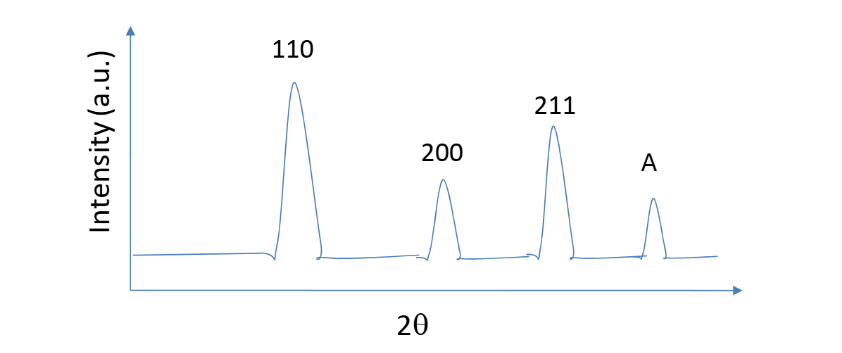
\includegraphics[width=0.5\linewidth]{figs/image1'.png}
    \caption{}
    \label{fig:placeholder}
\end{figure}

\begin{multicols}{2}
\begin{enumerate}
\item 210
\item 221
\item 211
\item 310
\end{enumerate}
\end{multicols}
\hfill(GATE MT 2016)

\item Which of the following cooling curves (shown in schematic) in an eutectoid steel will produce $50\%$ bainitic structure?

\begin{figure}[H]
    \centering
    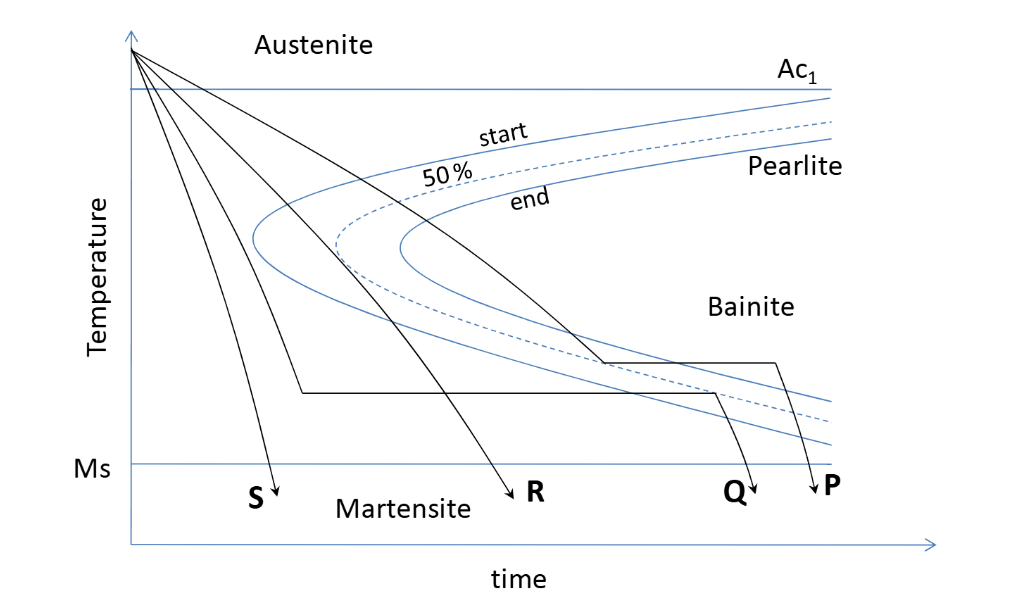
\includegraphics[width=0.5\linewidth]{figs/image2'.png}
    \label{fig:placeholder}
\end{figure}

\begin{multicols}{4}
\begin{enumerate}
\item P
\item Q
\item R
\item S
\end{enumerate}
\end{multicols}
\hfill(GATE MT 2016)

\item The Burger's vector of a dislocation in a cubic crystal (with lattice parameter \textbf{a}) is \brak{110} and dislocation line is along \brak{112} direction. The angle \brak{\text{in degrees}} between the dislocation line and its Burger's vector is

\item For the tensile stress-strain curve of a material shown in the schematic, the resilience (in MPa) is

\begin{figure}[H]
    \centering
    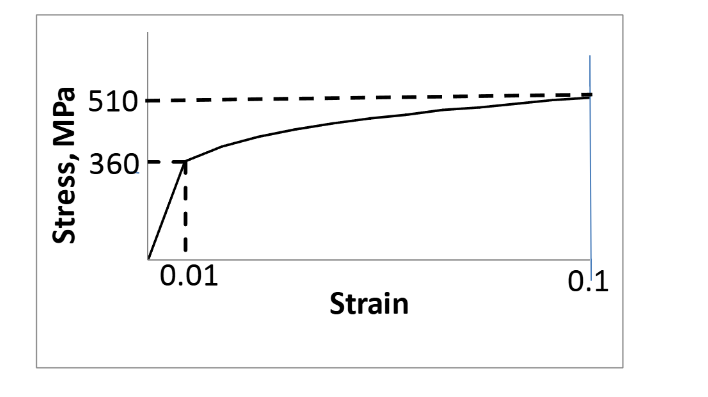
\includegraphics[width=0.5\linewidth]{figs/image3'.png}
    \caption{}
    \label{fig:placeholder}
\end{figure}

\item A plastically deformed metal crystal at low temperature exhibits wavy slip line pattern due
to
\begin{multicols}{2}
\begin{enumerate}
\item Dislocation pile-up
\item Large number of slip systems
\item Low stacking fault energy
\item Dislocation climb
\end{enumerate}
\end{multicols}
\hfill(GATE MT 2016)

\item Creep resistance decreases due to
\begin{multicols}{2}
\begin{enumerate}
\item Small grain size
\item Fine dispersoid size
\item Low stacking fault energy
\item High melting point
\end{enumerate}
\end{multicols}
\hfill(GATE MT 2016)

\item The operation NOT associated with casting is
\begin{multicols}{2}
\begin{enumerate}
\item Gating
\item Stack Moulding
\item Fettling
\item Calendaring
\end{enumerate}
\end{multicols}
\hfill(GATE MT 2016)

\item Of the following welding processes  

\begin{tabular}{ll}
{[P]} & Laser Beam Welding \\
{[Q]} & Submerged Arc Welding \\
{[R]} & Metal Inert Gas Welding \\
\end{tabular}

the width of the heat-affected zone in decreasing order is
\begin{enumerate}
\item P $>$ Q $>$ R
\item Q $>$ R $>$ P
\item R $>$ P $>$ Q
\item P $>$ R $>$ Q
\end{enumerate}
\hfill(GATE MT 2016)

\item Railway tracks are typically manufactured using
\begin{multicols}{4}
\begin{enumerate}
\item Forging
\item Extrusion
\item Deep Drawing
\item Rolling
\end{enumerate}   
\end{multicols}
\hfill(GATE MT 2016)


\item For dye-penetrant test, identify the \textbf{CORRECT} statement
\begin{enumerate}
\item Pre- and post-cleaning of parts are not required
\item Internal defects can be detected
\item Surface oxides helps in crack identification
\item Dye with low contact angle is required
\end{enumerate}
\hfill(GATE MT 2016)

\item Aluminium powder having an apparent density of 810 kg.m$^{-3}$ is compacted in a cylindrical die at 600 MPa. The density of the as-pressed aluminium compact is 1755 kg.m$^{-3}$. If the height of the as-pressed compact is 12 mm, the fill height (in mm) required is 
\hfill(GATE MT 2016)

\item A rolling mill has a roll diameter of 200 mm. If coefficient of friction is 0.1, then the maximum possible reduction (in mm) during rolling of a 250 mm thick plate is 
\hfill(GATE MT 2016)

\item A hot body cools according to the following equation

$$\frac{dT}{dt} = -cT$$

where, T is the instantaneous temperature at time t, and the constant $c = 0.05 \, s^{-1}$. Reduce the differential equation into its finite difference form \textbf{using forward difference}. For maintaining numerical stability, the maximum value of the time step $\Delta t$ (in seconds) is 
\hfill(GATE MT 2016)

\item Solve the equation $x = e^{-x}$ using Newton-Raphson method. Starting with an initial guess value $x_0 = 0$, the value of $x$ after the first iteration is 
\hfill(GATE MT 2016)

\item A coin is tossed three times. It is known that out of the three tosses, one is a \textbf{HEAD}. The probability of the other two tosses also being \textbf{HEADs} is 
\hfill(GATE MT 2016)

\item The vector parallel to the plane $3x - 2y + z = -1$ is
\begin{enumerate}
\item $\hat{i} + \hat{j} - \hat{k}$
\item $3\hat{i} - 2\hat{j} + \hat{k}$
\item $-\hat{i} + \hat{j} - \hat{k}$
\item $3\hat{i} - 2\hat{j} + 2\hat{k}$
\end{enumerate}
\hfill(GATE MT 2016)

\item The value of the integral

$$\int_{0}^{\pi/2} x \sin x \, dx =$$ 
\hfill(GATE MT 2016)

\item The grain sizes (in $\mu$m) measured at five locations in an alloy sample are: 16, 14, 18, 15 and 13. The mean, median and standard deviation of grain sizes respectively are (in $\mu$m)
\begin{enumerate}
\item 15.2, 15 and 1.7
\item 15.2, 15 and 1.9
\item 15.8, 15 and 1.9
\item 15.2, 16 and 1.7
\end{enumerate}
\hfill(GATE MT 2016)

\item The change of standard state from pure liquid to 1 wt.\% for Si dissolved in liquid Fe at 1873 K is expressed as

$$\mathrm{Si\ (liq.)} = \mathrm{Si\ (1\ wt.\%)}$$

Given that the activity coefficient of Si at infinite dilution in Fe is $10^{3}$, the standard Gibbs free energy change (in kJ) for this equilibrium is 
\hfill(GATE MT 2016)

\item The following experimental data are available for a hypothetical binary liquid system \textbf{A B} at 1073 K

\begin{tabular}{lccccc}
Atom fraction of A & 0.2 & 0.4 & 0.5 & 0.7 & 1.0 \\
Partial pressure of A (bar) & 0.01 & 0.04 & 0.06 & 0.07 & 0.08 \\
\end{tabular}

When the atom fraction of A is 0.4, the activity of A in the liquid is 
\hfill(GATE MT 2016)

\item The lining of a box-type furnace is made up of a refractory layer and steel plate as shown in the figure. Steady state temperature at the surface of the refractory is $1273$ K and that at the outer steel surface is $473$ K. If the steady-state heat flux through the refractory-steel plate composite is 1600 $W.m^2$, and heat flow is along x-direction, the thermal contact resistance ($W^{-1}.m2K$) between refractory and steel is
\begin{figure}[H]
    \centering
    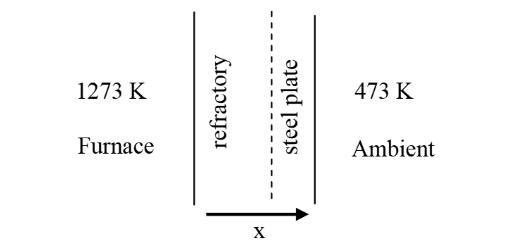
\includegraphics[width=0.5\linewidth]{figs/image4'.png}
    \caption{}
    \label{fig:placeholder}
\end{figure}

    Given data:\\
    Thermal conductivity of refractory: 1.2 $W.m^{-1}K^{-1}$\\
    Thickness of refractory lining: 80 $mm$\\
    Thermal conductivity of steel: 32 $W.m^{-1}K^{-1}$\\
    Thickness of steel plate: 4 $mm$
\hfill(GATE MT 2016)

\item The height of a liquid metal column in a cylindrical vessel is 3.2 m. At time t 0, liquid metal is drained out from the vessel through a small nozzle located at the base of the vessel. Neglecting frictional losses, the initial mass flow rate (in $kg.s^{-1}$) through the nozzle is 


    Given data:\\
    Density of liquid metal Nozzle diameter: 7000 kg \\
    Nozzle discharge coefficient: 30 mm
\hfill(GATE MT 2016)

\item Match entities listed in \textbf{Column I} with their correct dimensions given in \textbf{Column II}:

\begin{tabular}{ll}
\textbf{Column I} & \textbf{Column II} \\
{[P]} Drag coefficient & {[1]} M L$^{-1}$T$^{-1}$ \\
{[Q]} Mass transfer coefficient & {[2]} M L$^{-2}$T$^{-1}$ \\
{[R]} Viscosity & {[3]} M$^0$ L$^0$ T$^0$ \\
{[S]} Mass flux & {[4]} M$^0$ L T$^{-1}$ \\
\end{tabular}

\begin{enumerate}
\item P-3, Q-4, R-1, S-2
\item P-3, Q-1, R-2, S-4
\item P-1, Q-4, R-2, S-3
\item P-4, Q-3, R-1, S-2
\end{enumerate}
\hfill(GATE MT 2016)

\item Direct Reduced Iron (DRI) produced from a gas based process contains Fe, FeO, C and remainder being gangue. The chemical composition of DRI is: \textit{Total Fe = 92 wt.\% and Metallic Fe = 84 wt.\%}. The weight percent of FeO in DRI is 
\hfill(GATE MT 2016)

\item Mould heat flux ($q_m$) for billet casters is expressed (in SI unit) as a function of distance below the meniscus ($z$)

$$q_m(z) = \left[ 2.67 - 0.33 \sqrt{\frac{z}{U_c}} \right] \times 10^6 \qquad (0 \leq z \leq L_m)$$

If mould length ($L_m$) is 0.8 m and casting speed ($U_c$) is 0.2 m.s$^{-1}$, the average mould flux (in MW.m$^{-2}$) is 
\hfill(GATE MT 2016)

\item In BOF steelmaking, 5 metric ton of lime containing 90 wt.\% CaO is used to refine 100 metric ton of hot metal containing 93.2 wt.\% Fe. The slag produced during refining contains 40 wt.\% CaO and 22 wt.\% FeO. Neglecting material losses, the yield of Fe (in \%) is
\hfill(GATE MT 2016)

\item In vacuum degassing of steel, 14 ppm of dissolved nitrogen is in equilibrium with 1 mbar of nitrogen gas at 1873 K. At the same temperature, if the pressure is lowered to 0.7 mbar, the equilibrium nitrogen content (in ppm) is 
\hfill(GATE MT 2016)

\item During isothermal phase transformation (in solid-state), fraction transformed is measured at two different transformation times:
\begin{align}
    \begin{tabular}{|c|c|}
\hline
Transformation Time, $t$ (s) & Fraction Transformed, $f$ \\
\hline
75 & 0.11 \\
150 & 0.37 \\
\hline
\end{tabular}
\end{align}

Assuming Avrami kinetics $[f = 1 - \exp(-kt^n)]$, the fraction transformed in 300 seconds is 
\hfill(GATE MT 2016)

\item Zinc oxide is reduced at a constant temperature in a closed reactor using ZnO(s) and C(s) as the only starting materials. The following reactions are assumed to be at thermodynamic equilibrium:
\[
\text{ZnO(s) + C(s) = Zn(g) + CO(g)}
\]
\[
2CO(g) = CO_2(g) + C(s)
\]
Assume ideal gas behaviour. Based on mole balance, the relationship applicable to the system at equilibrium is
\begin{enumerate}
\item $p_{Zn} = p_{CO} + 2p_{CO_2}$
\item $p_{Zn} = 2p_{CO} + p_{CO_2}$
\item $p_{Zn} = p_{CO} + p_{CO_2}$
\item $p_{Zn} = 0.5p_{CO} + 2p_{CO_2}$
\end{enumerate}
\hfill(GATE MT 2016)

\item The critical nucleus size (in nm) when copper melt is under-cooled by 100 K is

Given data:\\  
Melting point: $1356$ K  \\
Density: $8900$ kg.m$^{-3}$  \\
Solid-liquid interfacial energy: $0.5$ Jm$^{-2}$ \\ 
Latent heat of freezing: $13000$ J.mol$^{-1}$  \\
Molar volume: $7$ $\times$10$^{-6}$ m$^{3}$mol$^{-1}$  

\begin{multicols}{4}
\begin{enumerate}
\item $0.36$  
\item $1.55$  
\item $3.65$  
\item $7.30$  
\end{enumerate}
\end{multicols}
\hfill(GATE MT 2016)

\item The density and corresponding crystallinity of two poly-propylene material are given below

\begin{center}
\begin{tabular}{|c|c|}
\hline
Density, kg.m$^{-3}$ & Crystallinity, \% \\
\hline
904 & 62.8 \\
895 & 54.4 \\
\hline
\end{tabular}
\end{center}

The density of totally amorphous poly-propylene (in kg.m$^{-3}$) is:

\begin{multicols}{4}
\begin{enumerate}
\item 723  
\item 841  
\item 905  
\item 956  
\end{enumerate}
\end{multicols}
\hfill(GATE MT 2016)

\item A simplified energy band-diagram of an intrinsic semiconductor at thermal equilibrium (300 K) is shown. In the accompanying table, which one of the four columns correctly represents the listed parameters? Assume same effective mass for electrons and holes.

\begin{figure}[H]
    \centering
    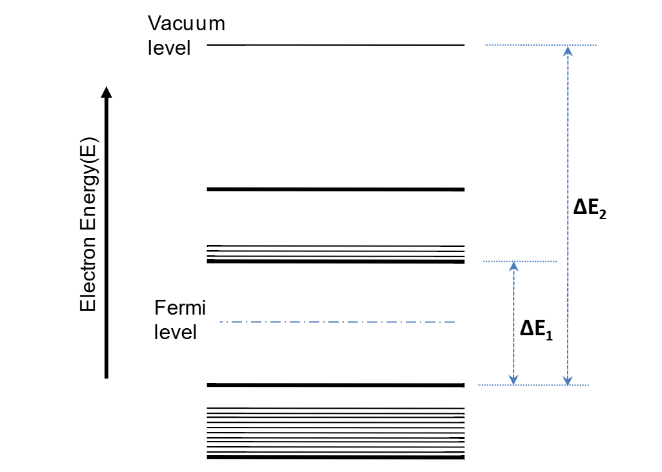
\includegraphics[width=0.5\linewidth]{figs/image5'.png}
    \caption{}
    \label{fig:placeholder}
\end{figure}

\begin{center}
\begin{tabular}{|c|c|c|c|c|}
\hline
Parameter & Column 1 & Column 2 & Column 3 & Column 4 \\
\hline
Band-gap & $\Delta E_{1}$ & $\Delta E_{1}$ & $\Delta E_{2}$ & $\Delta E_{1}$ \\
Electron affinity & $\Delta E_{2}/2$ & $\Delta E_{1}$ & $\Delta E_{2}/2$ & $\Delta E_{1} - (\Delta E_{2}/2)$ \\
Work function & $\Delta E_{1} + \Delta E_{2}$ & $\Delta E_{2} - (\Delta E_{1}/2)$ & $\Delta E_{1} - \Delta E_{2}/2$ & $\Delta E_{2} + (\Delta E_{1}/2)$ \\
\hline
\end{tabular}
\end{center}

\begin{multicols}{4}
\begin{enumerate}
\item Column 1
\item Column 2
\item Column 3
\item Column 4
\end{enumerate}
\end{multicols}
\hfill(GATE MT 2016)

\item A binary phase diagram is shown in the schematic.

\begin{figure}[H]
    \centering
    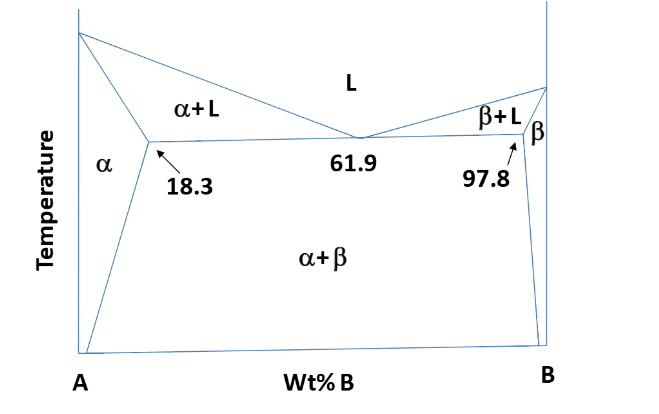
\includegraphics[width=0.5\linewidth]{figs/image6'.png}
    \caption{}
    \label{fig:placeholder}
\end{figure}

Upon complete solidification of a binary alloy system A-B, the fraction of pro-eutectic $\alpha$-phase present is 0.50. The alloy composition in terms of wt\% B is:
\hfill(GATE MT 2016)

\item Fatigue behaviour of an aluminium alloy is shown in the S N plot. A piston rod made of this material is subjected to:  
(i) 1000 cycles at 420 MPa, followed by  
(ii) 1000 cycles at 300 MPa.  
\begin{figure}[H]
    \centering
    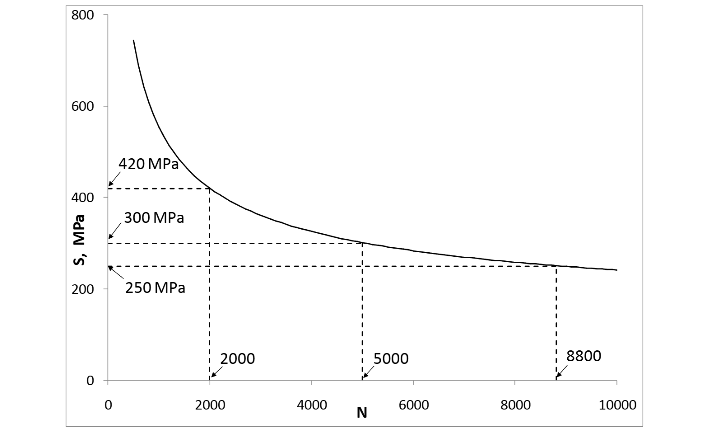
\includegraphics[width=1\linewidth]{figs/image7'.png}
    \caption{}
    \label{fig:placeholder}
\end{figure}

Using Miner\textquotesingle s rule of cumulative damage, the remaining fatigue life (in terms of number of cycles) at stress of 250 MPa is
\hfill(GATE MT 2016)

\item A glass plate has two parallel cracks. One of them is an internal crack of length 5 $\mu$m and the other is a surface crack of length 3 $\mu$m. A tensile stress is applied perpendicular to the crack surfaces. The fracture stress (in MPa) is  

\noindent Given data (for glass plate):\\  
Young\textquotesingle s Modulus = $70$ GPa \\ 
Surface energy per unit area = $1$ J.m$^{-2}$  
\hfill(GATE MT 2016)

\item A tensile stress is applied along the [100] direction in a FCC metal crystal. The critical resolved shear stress is 6 MPa. The tensile stress (in MPa) required for initiating slip on the (111) slip plane is
\hfill(GATE MT 2016)

\item For a bcc metal the ratio of the surface energy per unit area of the (100) plane to that of the (110) plane is 
\hfill(GATE MT 2016)

\item For a polymer reinforced with 40 vol.\% glass fiber, the elastic modulus (in GPa) along the transverse direction is  

\begin{multicols}{4}
\begin{enumerate}
\item 5.6  
\item 8.1  
\item 30.1  
\item 43.4  
\end{enumerate}
\end{multicols}

\noindent [E$_{\text{glass fiber}}$ = 70 GPa; E$_{\text{polymer}}$ = 3.5 GPa]
\hfill(GATE MT 2016)

\item In a sand-mould, a sprue of 0.25 m height and a top cross-section area of 2.2 m$^{2}$ is provided to maintain the melt flow rate at 4 m$^{3}$s$^{-1}$. To prevent aspiration of molten metal, the maximum cross-section area (in m$^{2}$) at the base of the sprue is 
\hfill(GATE MT 2016)

\item For casting a cylindrical aluminum bloom having a length of 1000 mm and diameter of 750 mm, the approximate solidification time (in minutes) estimated using Chvorinov\textquotesingle s rule is

\begin{multicols}{4}
\begin{enumerate}
\item 45  
\item 316  
\item 440  
\item 620  
\end{enumerate}
\end{multicols}

\noindent [The mould constant is 2 s/mm$^{2}$]
\hfill(GATE MT 2016)

\item A liquid phase sintered SiC-Ni composite has a solid-solid grain boundary energy ($\gamma_{\text{SiC-SiC}}$) of 0.80 J.m$^{-2}$ and a solid-liquid ($\gamma_{\text{SiC-Ni}}$) interfacial energy of 0.45 J.m$^{-2}$. For a SiC grain size of 20 $\mu$m, the average interparticle (SiC-SiC) neck size (in $\mu$m) is:

\begin{multicols}{4}
\begin{enumerate}
\item 3.03  
\item 4.28  
\item 9.16  
\item 18.32  
\end{enumerate}
\end{multicols}
\hfill(GATE MT 2016)

\item Match the deformation processes in Column I with the corresponding stress states listed in Column II  

\begin{center}
\begin{tabular}{|c|c|c|}
\hline
Column I & Column II\\
\hline
Wire Drawing & [1] Direct Compression \\
Forging & [2] Indirect Compression \\
Stretch Forming & [3] Tension \\
Cutting & [4] Shear \\
\hline
\end{tabular}
\end{center}

\begin{multicols}{2}
\begin{enumerate}
\item P-1; Q-2; R-3; S-4  
\item P-1; Q-2; R-4; S-3  
\item P-2; Q-1; R-3; S-4  
\item P-2; Q-1; R-4; S-3  
\end{enumerate}
\end{multicols}
\hfill(GATE MT 2016)




\end{enumerate}

\end{document}
